\section{Introduction}
\label{sec:intro}

Wide-field optical surveys such as the Zwicky Transient Facility \citep[ZTF;][]{bellm2019ztf} discover far more transients than spectroscopic facilities can follow up \citep{fremling2020bts,perley2020bts}.
Allocating telescope time from the first few nights of photometry depends on two coupled inferences: \emph{what} the object is and \emph{how bright} it will be.
FLARE \citep{sasli2026forecast,sasli2026flare} supplies both on ZTF: its hierarchical classifier assigns probabilities over six types---SN~Ia, core-collapse SN (CC~SN), superluminous SN (SLSN), AGN, tidal disruption event (TDE), and cataclysmic variable (CV)---while LightGBM quantile models forecast $g$- and $r$-band magnitudes from origins 5--30 days post-detection with 68\% and 95\% conformal bands.

\begin{figure*}[t]
\centering
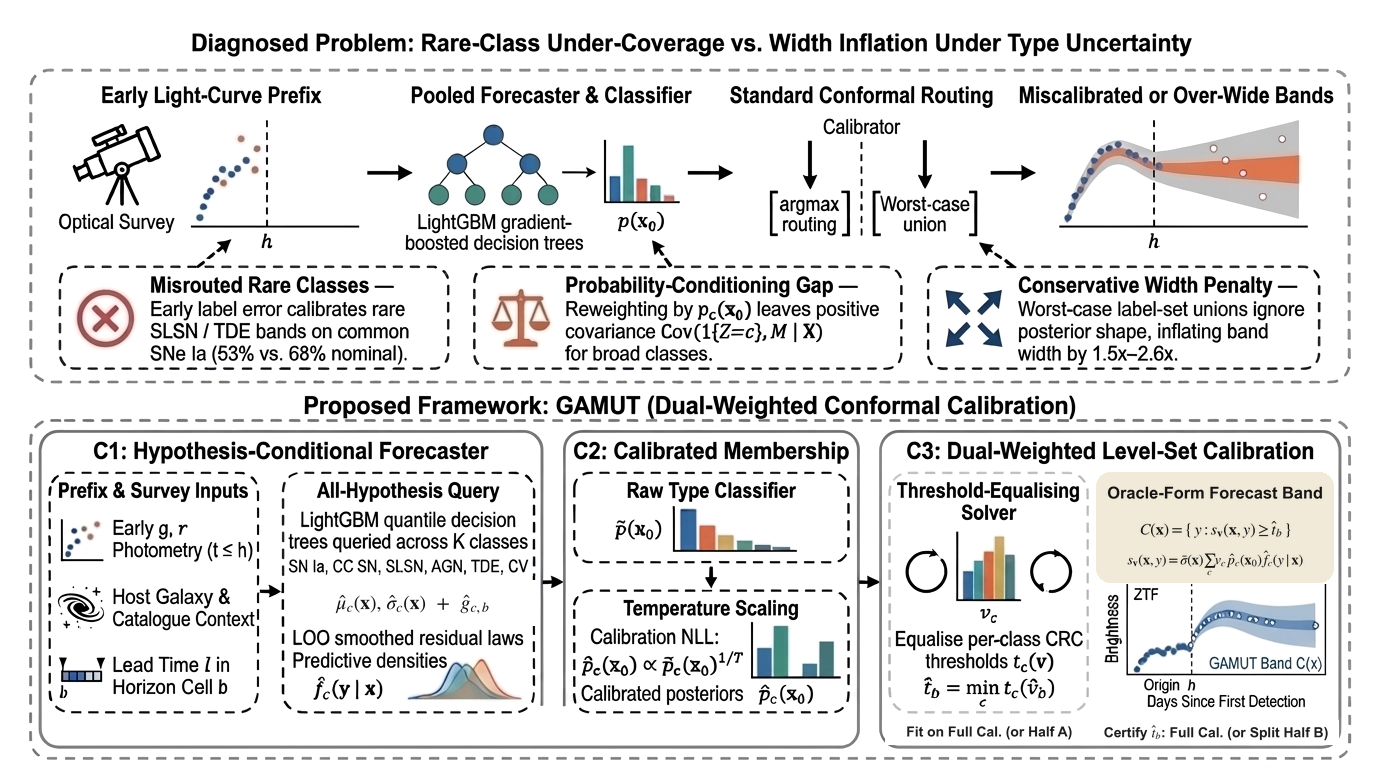
\includegraphics[width=0.97\textwidth]{figures/gamut_framework.png}
\vspace{-4pt}
\caption{Overview of \gamut{} and calibration failure modes under latent type uncertainty. \textbf{Top:} Routing multipliers by the early argmax class under-covers misclassified rare transients, probability reweighting leaves a positive covariance gap (\cref{prop:gap}), and worst-case unions inflate band width across common sources. \textbf{Bottom:} \gamut{} queries a shared hypothesis-conditional quantile forecaster and leave-one-object-out residual laws across all $K$ classes (\textbf{C1}), temperature-scales raw type posteriors (\textbf{C2}), and solves a multiplicative fixed point to equalise per-class conformal risk-control thresholds (\textbf{C3}), outputting level-set bands $C(x)$. Curves and icons are schematic.}
\label{fig:gamut-overview}
\vspace{-4pt}
\end{figure*}

While FLARE's bands achieve nominal marginal coverage across the SN~Ia-dominated stream, they systematically under-cover the rare classes most valuable for follow-up: five days after first detection, the 68\% band contains only \ZTFflareSLSNsixtyeight{} of future SLSN measurements, alongside substantial shortfalls for TDEs and CVs (\cref{fig:observation}).
The cause is structural: routing conformal multipliers by the \emph{predicted} class calibrates misclassified rare transients against common-supernova residuals.
The same mismatch arises across clinical subtyping, regime monitoring, and multi-source sensing whenever calibration data carry ground-truth group labels that remain latent at test time.

Existing remedies force a choice between rare-class under-coverage and excessive width (\cref{fig:gamut-overview}, top).
Conditioning on classifier \emph{probabilities}---via conditional-guarantee conformal prediction \citep{gibbs2025conformal}, posterior localisation \citep{guan2023localized}, or label-shift mixtures \citep{podkopaev2021distribution}---controls a probability-weighted moment rather than true-class coverage.
By \cref{prop:gap}, the two differ by the conditional covariance between class membership and miscoverage plus posterior error; whenever a rare class exhibits broader forecast residuals than the classes with which it is confused, this covariance is positive and sustains under-coverage.
Conversely, latent-class-valid constructions---the max-class quantile \citep{barber2021limits}, two-step label-set unions \citep{timans2024adaptive}, and multi-distribution CP \citep[MDCP;][]{yang2026multi}---ignore or coarsen posterior shape, inflating widths by $1.5\times$--$2.6\times$.

To resolve this tension, we derive the population-optimal band (\cref{prop:oracle}): the set of minimal scale-weighted length satisfying per-class coverage constraints is a superlevel set of $\bar\sigma(x)\sum_c v_c\,p_c(x)f_c(y\mid x)$, with posterior $p_c(x)$, class-$c$ predictive density $f_c(y\mid x)$, posterior-mean scale $\bar\sigma(x)$, and dual weights $v_c$ up-weighting hard-to-cover classes.
\gamut{} (\emph{Guarantees for All Members Under Type uncertainty}; \cref{fig:gamut-overview}, bottom) estimates this oracle via three modules:
\begin{itemize}\setlength{\itemsep}{1pt}\setlength{\parskip}{0pt}\setlength{\topsep}{2pt}
\item[\textbf{C1}] \textbf{Hypothesis-conditional forecaster:} shared LightGBM quantile trees queried across all $K$ hypotheses paired with leave-one-object-out smoothed residual laws $\hat f_c(y\mid x)$, letting rare classes borrow cadence and colour structure from common ones;
\item[\textbf{C2}] \textbf{Calibrated membership posterior:} temperature-scaled probabilities $\hat p_c(x_0)$ fitted on calibration labels;
\item[\textbf{C3}] \textbf{Dual-weighted level-set calibration:} a multiplicative fixed point adjusting $v_c$ to equalise per-class conformal risk-control thresholds across adaptive horizon cells, keeping the minimum eligible threshold.
\end{itemize}
Under FLARE's cross-conformal protocol, \gamut{} reuses out-of-fold calibration data to approximate the oracle empirically.
Under a strict train/calibration/test split reserving a disjoint calibration half for threshold certification (\cref{thm:valid}), the identical rule guarantees finite-sample coverage for every class--horizon cell with sufficient certification objects, regardless of posterior or density misspecification.

\paragraph{Contributions.}
(i) An exact coverage-gap decomposition showing why predicted-class and probability-conditioned calibration under-cover hard rare classes (\cref{prop:gap}), validated on ZTF-BTS.
(ii) Characterisation of the shortest scale-weighted class-valid band (\cref{prop:oracle}), the \gamut{} estimator (\cref{alg:gamut}), and its strict-split finite-sample guarantee (\cref{thm:valid}).
(iii) Evaluation across ZTF-BTS, PLAsTiCC, three UCR archives, a synthetic suite, a strict ZTF split, and two pre-registered untouched PLAsTiCC WFD chunks against 13 baselines: on ZTF, conservative valid baselines are \ZTFValidOverFlareSixtyeight{} (68\%) and \ZTFValidOverFlareNinetyfive{} (95\%) wider than FLARE, whereas \gamut{} achieves class validity at \ZTFWidthRatioSixtyeight{} and \ZTFWidthRatioNinetyfive{} times FLARE's width (\StrictWidthGamutSixtyeight{} and \StrictWidthGamutNinetyfive{} under the strict split) and is \SynValidOverGamutSixtyeight{} (68\%) and \SynValidOverGamutNinetyfive{} (95\%) narrower than valid baselines on synthetic data.
(iv) A learned next-detection simulation with Venn--Abers recalibration that sharpens FLARE's set-closure probabilities.
